\chapter{Assegnare una Probabilità con $\Omega$ Qualsiasi}
In questo capitolo cercheremo di affrontare la casistica in cui il nostro spazio campionario non sia per forza discreto, come fatto in precedenza. Per aiutarci in ciò, distingueremo due casistiche: un caso \textit{"semplice"} ed un caso più complesso con $\Omega \subseteq \mathbb{R}$.
\section{Caso ``Semplice": Classi di Eventi}\label{sec:caso-semplice}
In questa trattazione avremo sì $\Omega$ generico, ma ci interesserà solo una classe ristretta di eventi $\mathcal{C}$, che quindi contiene sottoinsiemi di $\Omega$.
\begin{definizione}
    Data $\mathcal{C}\in \mathcal{P}(\Omega)$ una classe (o famiglia) di sottoinsiemi si definisce $\sigma(\mathcal{C})$ la più piccola $\sigma$-algebra che contiene $\mathcal{C}$, e la si denota con "$\sigma$-algebra generata dalla classe $\mathcal{C}$"
\end{definizione}
\begin{proposizione}
    Per qualsiasi classe $\mathcal{C}$ di sottoinsiemi di $\Omega$, esiste sempre $\sigma(\mathcal{C})$
\end{proposizione}

Si osservi che anche se $\mathcal{C} \subseteq \mathcal{P}(\Omega)$ (dove l'insieme delle parti è una $\sigma$-algebra), questo non implica che $\mathcal{C}$ contenga una $\sigma$-algebra di $\Omega$.\\
\\
Per costruire $\sigma(\mathcal{C})$ si parte dall'insieme $\mathcal{F}$ definito come: $\mathcal{F} = \{\mathcal{A}_\alpha: \mathcal{A}_\alpha\supseteq\mathcal{C}\}$, ovvero l'insieme che contiene tutte le $\sigma$-algebre che contengono $\mathcal{C}$. A questo punto, la $\sigma$-algebra generata da $\mathcal{C}$ risulta essere
\[\sigma(\mathcal{C}) = \bigcap_\alpha \mathcal{A}_\alpha\]
Dove l'intersezione rimane una $\sigma$-algebra ed è per costruzione la più piccola.
\begin{definizione}
    Si dice che $\;\mathcal{C} = \{C_k: k\in I\}\subseteq \mathcal{P}(\Omega)$ è una partizione discreta di $\Omega$ se:
    \begin{enumerate}
        \item $I\subseteq\mathbb{N}$ \hfill \textit{(ossia che $I$ è finito o al più numerabile)}
        \item $C_k \cap C_h = \varnothing \quad \forall h\neq k$
        \item $\bigcup_{k\in I} C_k = \Omega$
    \end{enumerate}
\end{definizione}

Si presti attenzione che $\mathcal{C}$ è  una famiglia di insiemi $C_k$ (visti come insiemi unici), tuttavia se faccio l'unione di (per esempio) $C_1\cup C_2$, questo potrebbe non stare in $\mathcal{C}$.\\
\\
Da un punto di vista modellistico, partizionare $\Omega$ ci permette di far "realizzare" almeno un (ed uno solo, in quanto sono disgiunti) evento della classe $\mathcal{C}$.
\begin{figure}[H]
    \centering
    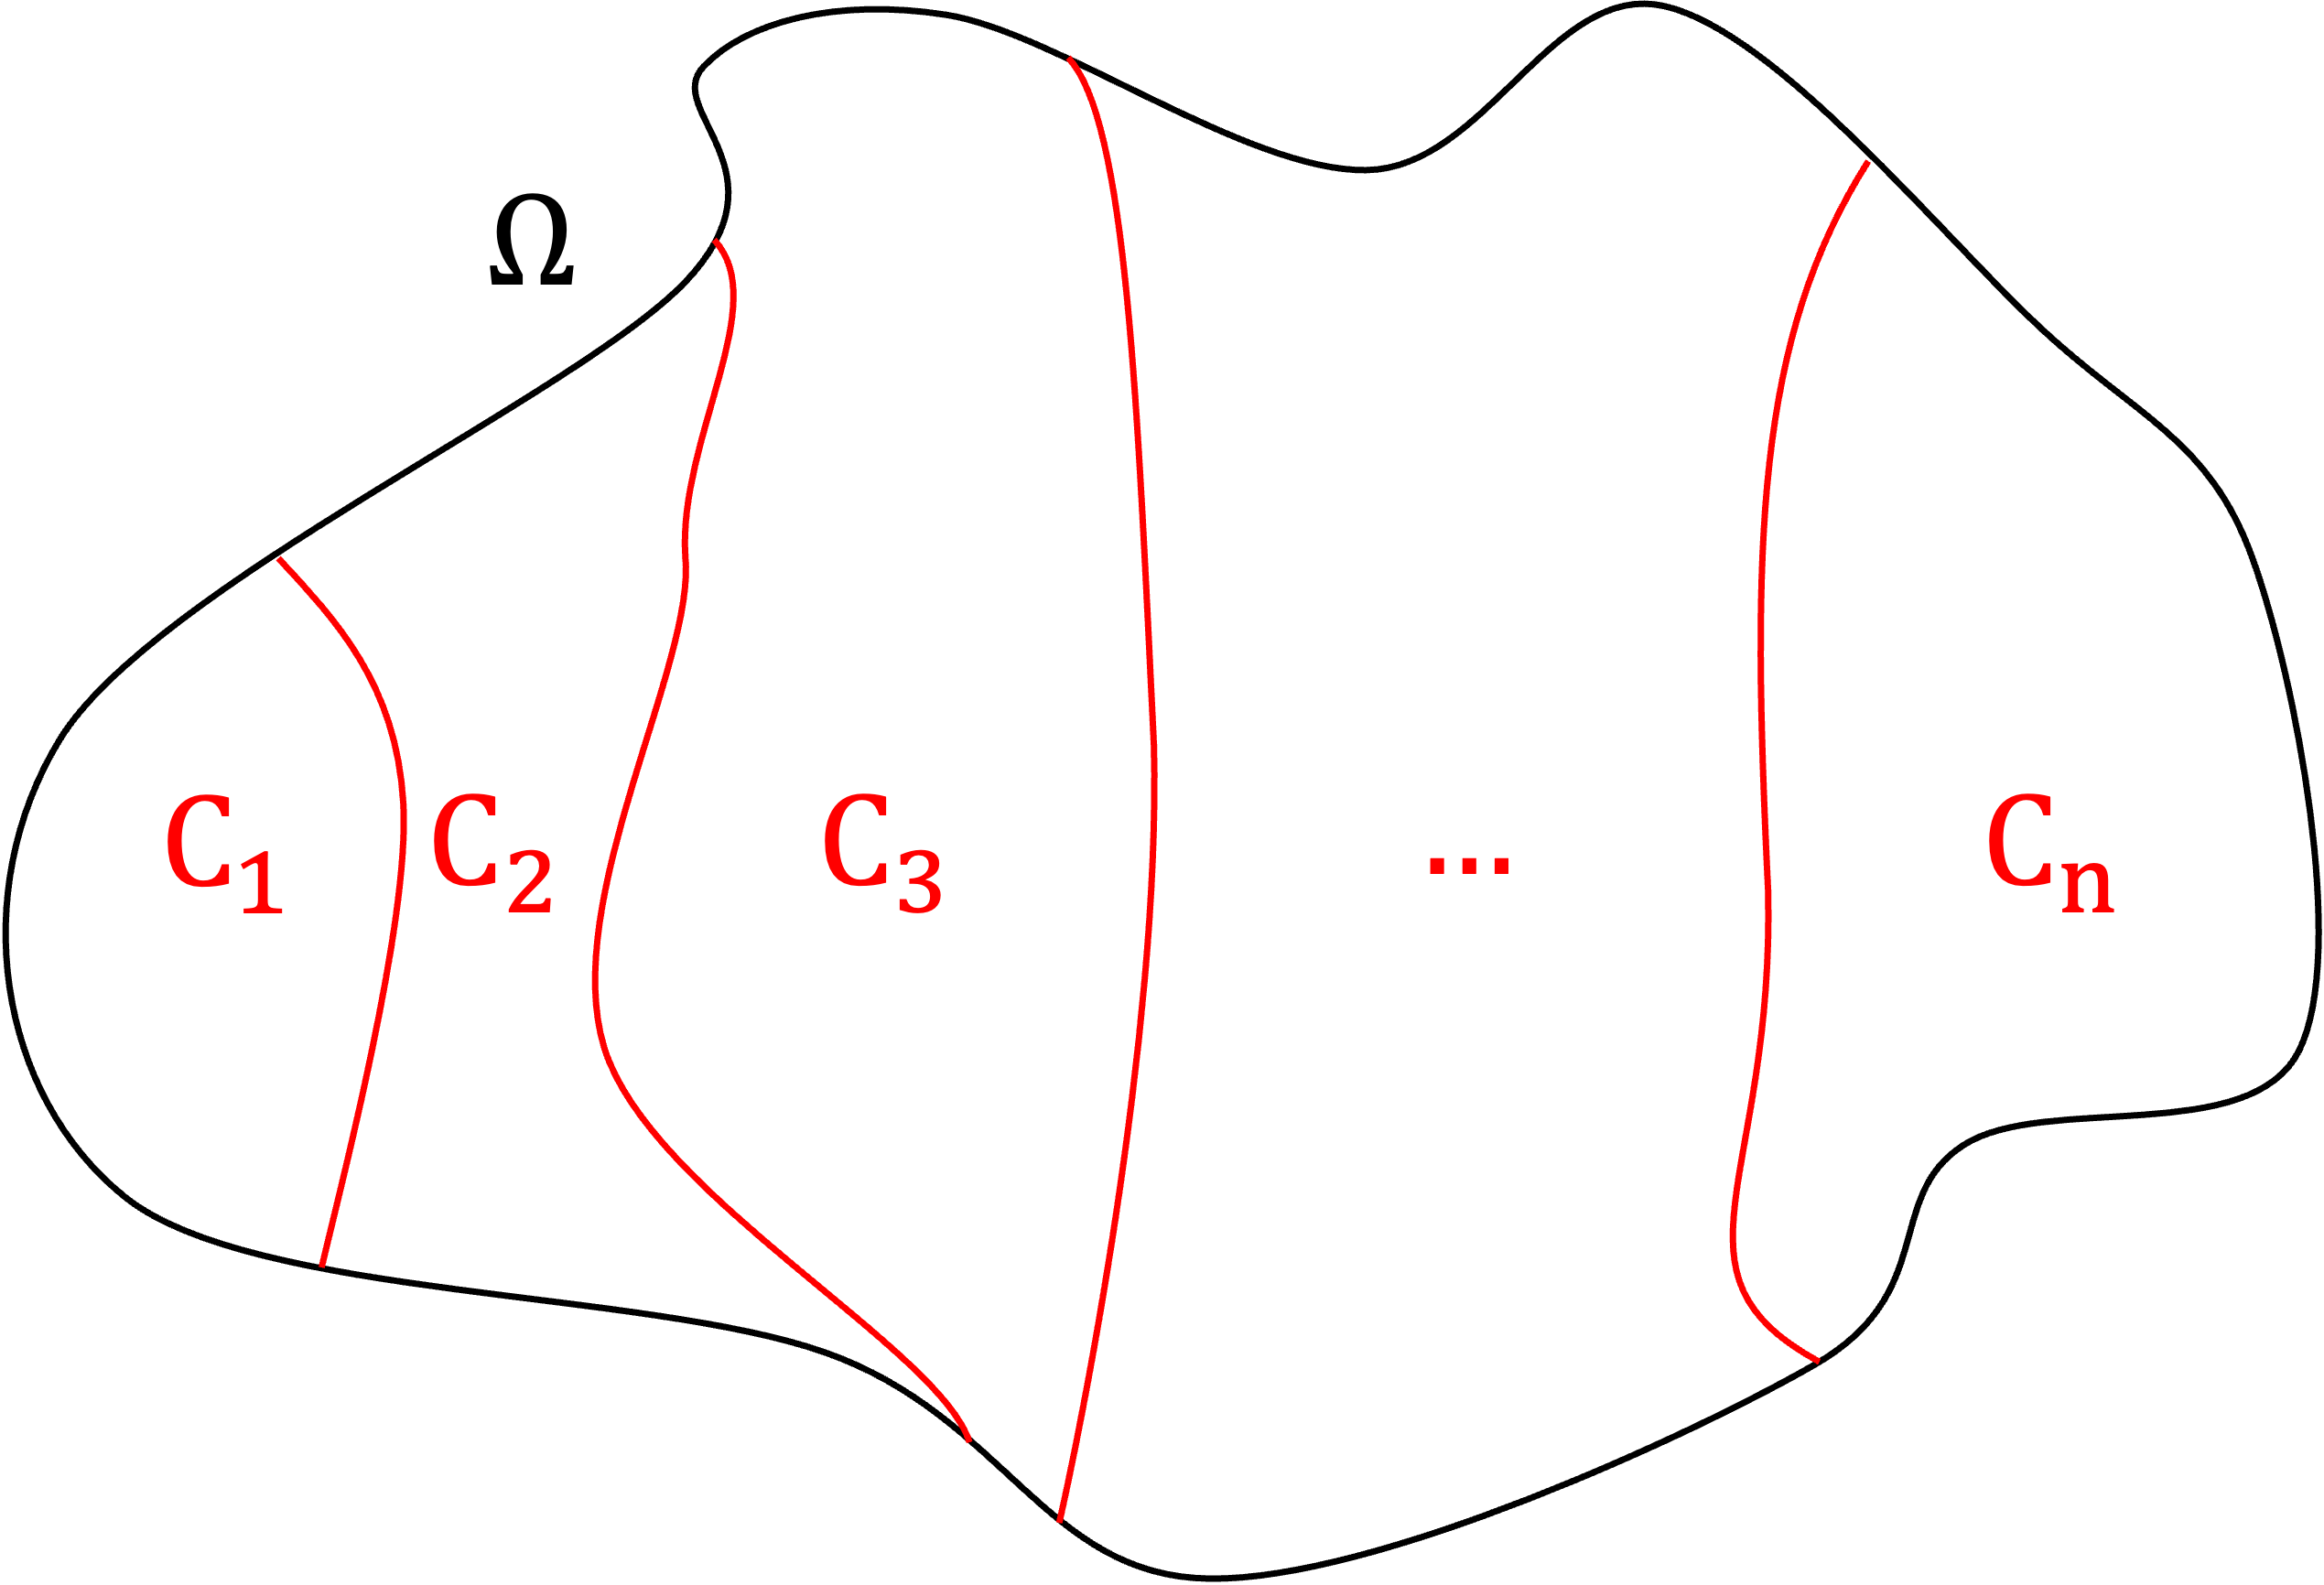
\includegraphics[width=0.3\linewidth]{Media/Partizione.png}
    \caption{Esempio grafico di una partizione}
    \label{fig:placeholder}
\end{figure}

\begin{esempio}
    Consideriamo $\mathbb{R}^+ = \bigcup_{n=1}^\infty[n-1, n)\;$ con $\;C_n = [n-1, n)$. \\Allora $\;\mathcal{C} =\{ C_n: n\in[1, + \infty)\}$ è una partizione di $\mathbb{R}^+$ diversa da $\mathcal{P}(\Omega)$. Siamo quindi riusciti ad isolare una classe al più numerabile.
\end{esempio}

\begin{proposizione}
    Quando $\mathcal{C}$ è una partizione discreta di $\Omega$, allora:
    \[\mathcal{A} = \sigma (\mathcal{C}) = \set{A \subseteq \Omega \quad| \quad A  = \bigcup_{j\in J}C_j, \quad J\subseteq I}\]
\end{proposizione}

Questa proposizione ci permette di vedere gli elementi della partizione come "atomi": in un certo senso sono l'unità più piccola. Non posso far altro che unire due elementi $C_h$ e $C_k$, non posso scindere in parti più piccole.

\begin{esempio}
    Nell'esempio precedente, posso solo dire quale intervallo si è \textit{acceso}, ma non ho un livello di dettaglio maggiore.
\end{esempio}
Abbiamo quindi capito che dato un $\Omega$ qualsiasi con $\mathcal{C}$ sua partizione discreta, allora ci conviene prendere $\mathcal{A} = \sigma (\mathcal{C})$. Ma come assegno $\mathbb{P}$?
\begin{teorema}
    Dato $\Omega$ qualsiasi e $\mathcal{C}$ una sua partizione discreta, allora:
    \begin{enumerate}
        \item Ogni $\mathbb{P}$ su $(\Omega, \sigma(\mathcal{C}))$ è univocamente determinata da 
        \[p_n = \mathbb{P}(C_n)\]
        Infatti $\forall A \in \sigma(\mathcal{C}), \quad A \overset{(3.4)}{=} \bigcup_{j\in J}C_j,\quad J\subseteq I:$
        \[\mathbb{P}(A) = \mathbb{P}\left(\bigcup_{j\in J}C_j\right) \overset{\sigma-add}{=} \sum_{j\in J}\mathbb{P}(C_j)  = \sum_{j \in J} p_j\]
        \item Data una successione $(p_n)_{n\geq1}$ di numeri reali, allora:
        \[
        \exists!\;\mathbb{P}:\sigma(\mathcal{C})\rightarrow[0, 1] \quad t.c. \quad \mathbb{P}(C_n) = p_n 
        \quad \iff \quad
        \begin{cases}
            p_n \geq 0 \quad \forall n\in I \\
            \sum_{n \in I} p_n = 1
        \end{cases}
        \]
    \end{enumerate}
\end{teorema}

\section{Probabilità Condizionata}

La probabilità (che di per se è una misura di quanto un evento è lecito pensare che accada), è influenzata dalla quantità di informazioni che abbiamo a disposizione. La probabilità condizionata misura quanto un evento A diventa probabile una volta che sappiamo che un altro evento B è accaduto.\\
\\
Non è più una probabilità “assoluta”, ma una probabilità relativa ad un contesto (o ad un'informazione aggiuntiva che abbiamo). \\
\\
Poniamoci nell'esperimento dove si lanciano 2 dadi, se volessimo calcolare la probabilità dell'evento $A =$ \textit{"la somma dei dadi è 12"}, allora potremmo calcolarla banalmente come $\mathbb{P}(A) = \frac{|A|}{|\Omega|} = 1/36$.\\
Se però consideriamo l'evento $E = $\textit{"Sul primo dado esce 6"}, e volessi capire $\mathbb{P}(A)$ dato che l'evento $E$ si è verificato, è come se $E$ "diventasse" il nostro "nuovo" $\Omega$.
\begin{figure}[H]
    \centering
    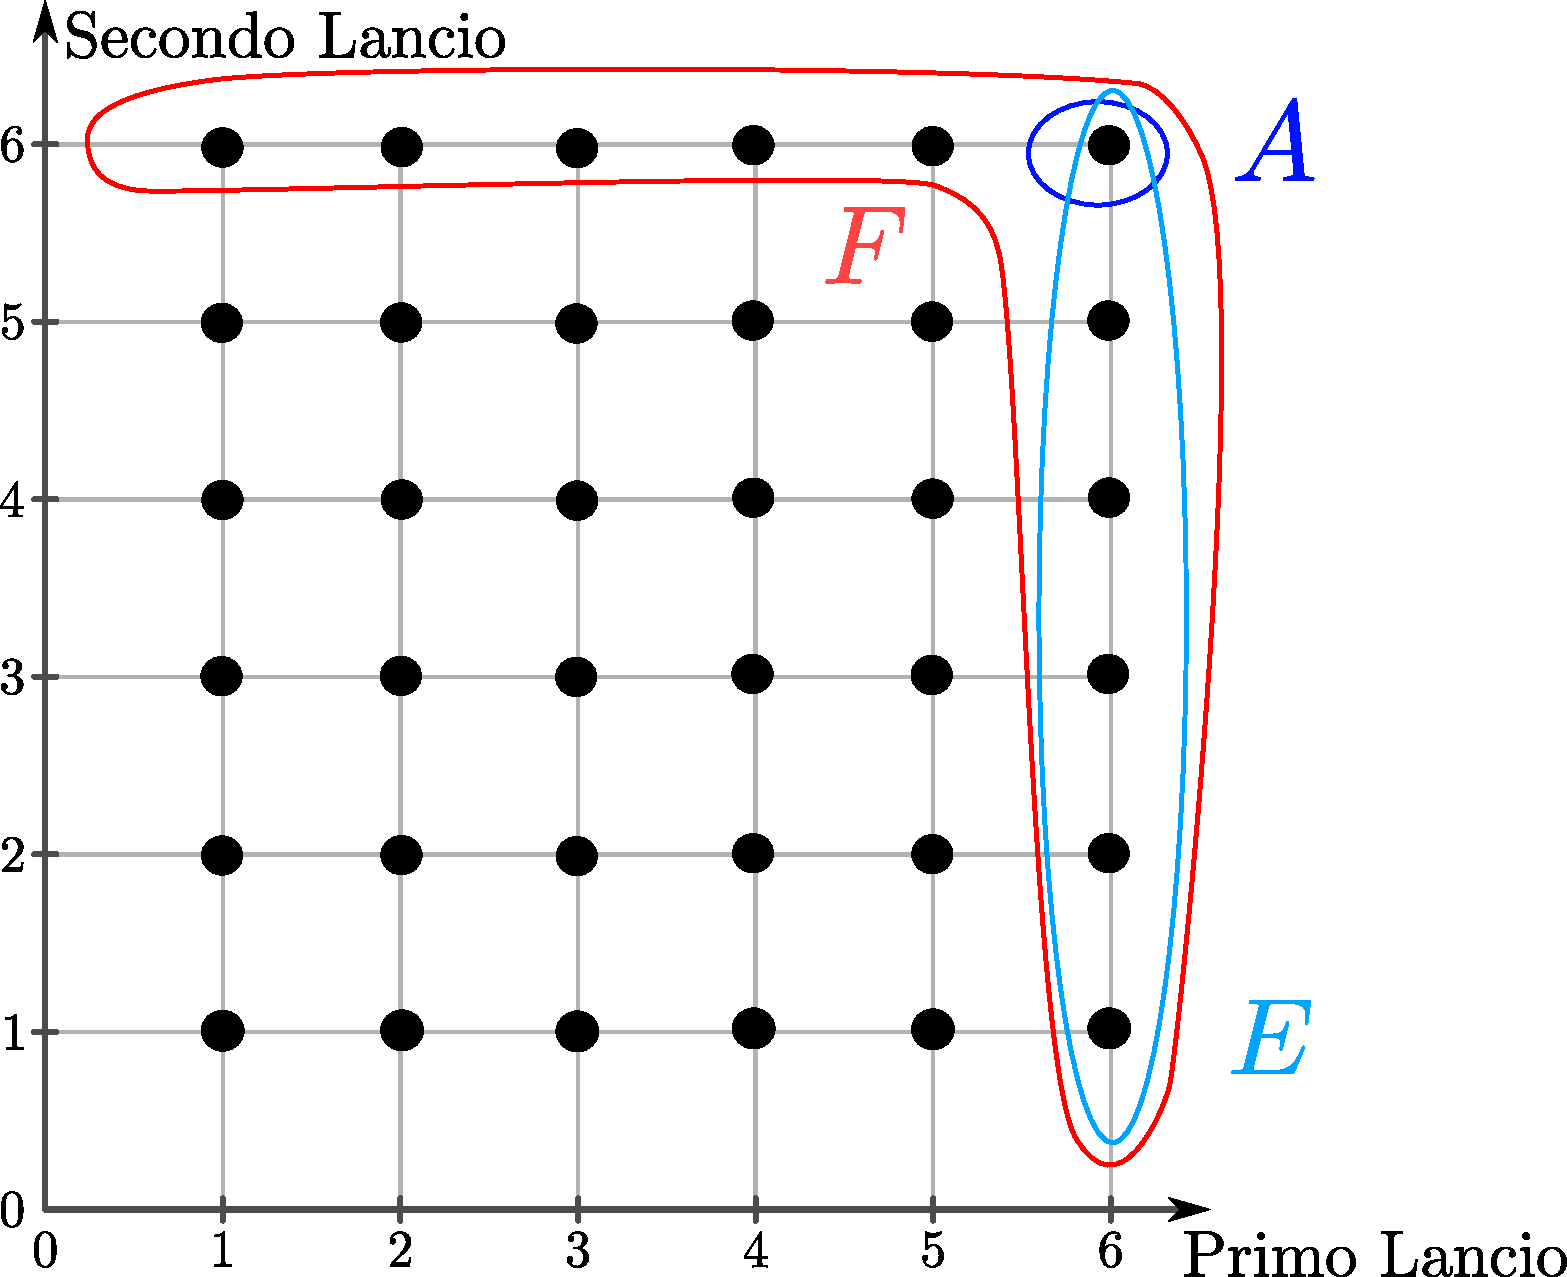
\includegraphics[width=0.4\linewidth]{Media/lanci.pdf}
\end{figure}
\noindent Come è facile intuire dal disegno avremo che la probabilità condizionata risulta essere:
\[\mathbb{P}(A \text{ "dato che si è verificato" }E) = \frac{|A\cap E|}{|E|} = \frac{|\{6, 6\}|}{6} = \frac{1}{6}\]
Se inoltre aggiungessimo l'evento $F = $ \textit{"Uno dei due dadi ha dato 6"}, ci aspetteremmo per buon senso che $\mathbb{P}(A \text{ "dato" }E) > \mathbb{P}(A\text{ "dato" }F)$, siccome sapere che si è verificato l'evento $E$ ci dà più informazioni rispetto all'evento $F$ (banalmente conosco su quale dei due dadi è uscito 6).\\
\\
Andiamo a formalizzare questi concetti in una solida teoria.

\begin{definizione}
    Dato $(\Omega, \mathcal{A}, \mathbb{P})$ spazio di probabilità e sia $E\subseteq \mathcal{A}$ un evento non trascurabile, i.e $\mathbb{P}(E) \gneq 0$. Allora $\forall A\in\mathcal{A}$ la probabilità condizionata di $A$ dato $E$ è il numero $\mathbb{P}(A|E)$:
    \[\mathbb{P}(A|E) = \frac{\mathbb{P}(A\cap E)}{\mathbb{P}(E)}\]
\end{definizione}
Dalla definizione vediamo immediatamente che è fondamentale che $\mathbb{P}(E)\neq 0$, altrimenti la scrittura non avrebbe senso matematico.\\
\\
Andando a riprendere l'esempio fatto precedentemente, ora che abbiamo un concetto formale di probabilità condizionata, e non più solo intuitivo, possiamo andare a calcolare le probabilità e confermare se i ragionamenti fatti in precedenza erano validi. \\
\[\mathbb{P} (A|E) = \frac{\mathbb{P}(A\cap E)}{\mathbb{P}(E)} = \frac{\mathbb{P}(\{6, 6\})}{\mathbb{P}\left(\{6, k\}; \;k\in\{1, ..., 6\}\right)} = \frac{\frac{|A\cap E|}{|\Omega|}}{\frac{|E|}{|\Omega|}} = \frac{|A\cap E|}{|E|} = \frac{1}{6}\]
Facendo lo stesso ragionamento con l'evento $F$:
\[\mathbb{P}(A|F) = \frac{\mathbb{P}(A \cap F)}{\mathbb{P}(F)} = \frac{|A\cap F|}{|F|} = \frac{1}{11} < \frac{1}{6}\]
dimostrando che l'intuizione che avevamo avuto sul fatto che $\mathbb{P}(A |E) > \mathbb{P}(A|F)$ era corretta.\\
\\
Osserviamo anche che dato un evento generico $E\in\mathcal{A}$ non trascurabile, allora possiamo definire $\mathbb{P}(A|E) = \frac{\mathbb{P}(A\cap E)}{\mathbb{P}(E)}$. Questo ci porta a dei casi limite:
\begin{itemize}
    \item Supponendo che $A\subseteq E:\quad \mathbb{P}(A|E) = \frac{\mathbb{P}(A\cap E)}{\mathbb{P}(E)} = \mathbb{P}(A|E) = \frac{\mathbb{P}(E)}{\mathbb{P}(E)} = 1$
    \item Se $A \text{ ed }E$ sono incompatibili\footnote{Ovvero che $E\cap A=\varnothing$}: $\quad\mathbb{P}(A|E) = 0$.
\end{itemize}

\begin{proposizione}
\label{prop:mappa_condizionata}
    Sia $E \in \mathcal{A}$ un evento non trascurabile. Allora la mappa:
    \[
    A \longmapsto \mathbb{P}(A \mid E) := \mathbb{P}_E(A)
    \]
    è una misura di probabilità su $\mathcal{A}\rightarrow [0,1]$.
\end{proposizione}
Questa proposizione ci permette di vedere la probabilità condizionata come una misura di probabilità, facendo così valere tutte le proprietà studiate sin ora.
\begin{esempio}
    Vale la proprietà $\quad \mathbb{P}(A^c|E) = 1 - \mathbb{P}(A|E)$, che scrivendola con la notazione più compatta diventa: $\quad \mathbb{P}_E(A^c) = 1 - \mathbb{P}_E(A) $
\end{esempio}
\bigskip
\noindent
\begin{tikzpicture}
  \draw[dashed] (0,0) -- (\textwidth,0);
\end{tikzpicture}\\
\\
Arrivati a questo punto vorremmo \textit{unire} i concetti di partizione e probabilità condizionata.\\
Vedremo infatti che si può partire da due partizioni di uno stesso spazio campionario $\Omega$, per ottenerne una terza, più \emph{fine}, che ne rappresenta tutte le possibili intersezioni. Inoltre, vorremo studiare come le probabilità associate a tali eventi intersezione possono essere calcolate a partire dalle probabilità condizionate.\\
\\
Possiamo rappresentare la struttura delle probabilità condizionate tramite un albero, in cui dal nodo radice $\Omega$ si diramano i rami verso gli eventi $A_n$, e da ciascun $A_n$ partono i sotto-rami verso gli eventi $B_k$.
\begin{center}
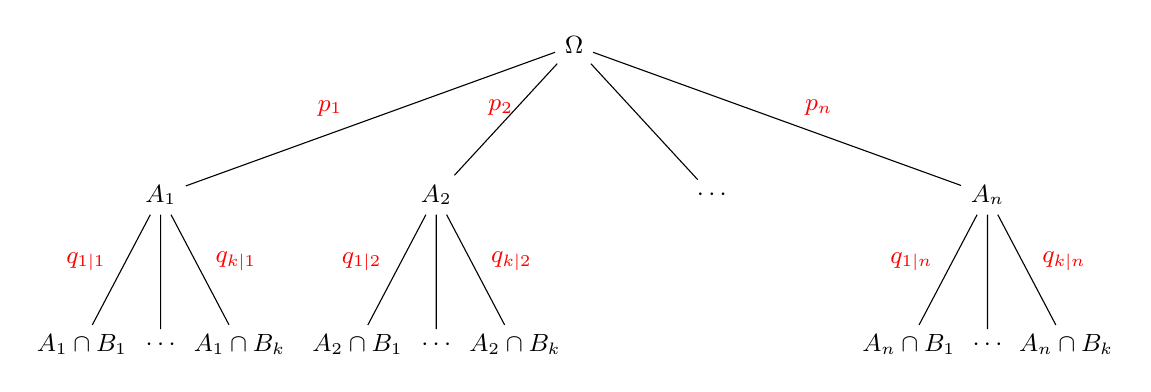
\begin{tikzpicture}[
  level distance=1.9cm,
  level 1/.style={sibling distance=35mm},
  level 2/.style={sibling distance=10mm},
  every node/.style={font=\small},
  edge from parent/.style={draw,-}
]
  % Nodo radice
  \node (root) {$\Omega$}
    % --- A1 ---
    child { node (A1) {$A_1$}
      child { node {$A_1 \cap B_1$}
              edge from parent node[pos=.60,above left] {\textcolor{red}{$q_{1|1}$}} }
      child { node {$\cdots$} }
      child { node {$A_1 \cap B_k$}
              edge from parent node[pos=.60,above right] {\textcolor{red}{$q_{k|1}$}} }
      edge from parent node[pos=.55,above left] {\textcolor{red}{$p_1$}}
    }
    % --- A2 ---
    child { node (A2) {$A_2$}
      child { node {$A_2 \cap B_1$}
              edge from parent node[pos=.60,above left] {\textcolor{red}{$q_{1|2}$}} }
      child { node {$\cdots$} }
      child { node {$A_2 \cap B_k$}
              edge from parent node[pos=.60,above right] {\textcolor{red}{$q_{k|2}$}} }
      edge from parent node[pos=.55,above] {\textcolor{red}{$p_2$}}
    }
    % --- puntini ---
    child { node {$\cdots$} }
    % --- An ---
    child { node (An) {$A_n$}
      child { node {$A_n \cap B_1$}
              edge from parent node[pos=.60,above left] {\textcolor{red}{$q_{1|n}$}} }
      child { node {$\cdots$} }
      child { node {$A_n \cap B_k$}
              edge from parent node[pos=.60,above right] {\textcolor{red}{$q_{k|n}$}} }
      edge from parent node[pos=.55,above right] {\textcolor{red}{$p_n$}}
    };
\end{tikzpicture}
\end{center}
Dove in rosso troviamo le probabilità degli eventi sottostanti, e per semplicità di notazione si è usato $\; q_{t|h} = \mathbb{P}(B_t|A_h)$.\\
\\
Ponendo la questione in maniera formale:
\\
Sia $(A_n : n \in I)$ una partizione discreta di $\Omega$ formata da eventi non trascurabili.
Analogamente, sia $(B_k:k \in I)$ un'altra partizione discreta dello stesso spazio campionario $\Omega$.
Ciascuna partizione suddivide $\Omega$ in eventi disgiunti e la loro unione ricopre tutto lo spazio.\\
\\
Dalle due partizioni possiamo ottenere una partizione \emph{più fine}, data dalle loro intersezioni:
\[
(A_n \cap B_k : n, k \in I),
\]
che costituisce ancora una partizione discreta di $\Omega$.
% --- DIAGRAMMA PARTIZIONE ---
\begin{center}
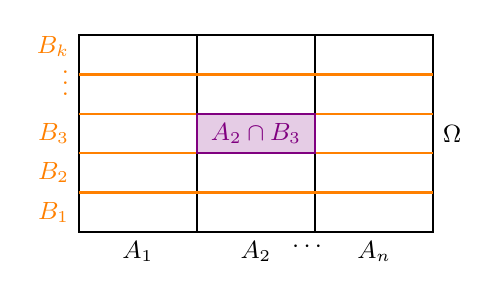
\begin{tikzpicture}[scale=0.5, every node/.style={font=\small}]
  % rettangolo esterno
  \draw[thick] (0,0) rectangle (9,5);
  \node[right] at (9,2.5) {$\Omega$};

  % linee verticali (partizione A)
  \foreach \x in {3,6}
    \draw[thick] (\x,0) -- (\x,5);

  % linee orizzontali (partizione B)
  \foreach \y in {1,2,3,4}
    \draw[orange, thick] (0,\y) -- (9,\y);

  % etichette A
  \node[below] at (1.5,0) {$A_1$};
  \node[below] at (4.5,0) {$A_2$};
  \node[below] at (5.8,0) {$\cdots$};
  \node[below] at (7.5,0) {$A_n$};

  % etichette B
  \node[left, orange] at (0,0.5) {$B_1$};
  \node[left, orange] at (0,1.5) {$B_2$};
  \node[left, orange] at (0,2.5) {$B_3$};
  \node[left, orange] at (0,4.0) {$\vdots$};
  \node[left, orange] at (0,4.7) {$B_k$};

  % rettangolo evidenziato per A2 ∩ B3
  \filldraw[fill=violet!20, draw=violet, thick] (3,2) rectangle (6,3);
  \node at (4.5,2.5) {\textcolor{violet}{$A_2 \cap B_3$}};
\end{tikzpicture}
\end{center}
Supponiamo di conoscere le probabilità
\(p_n = \mathbb{P}(A_n), \quad q_{k|n} = \mathbb{P}(B_k \mid A_n).\)\\
\\
La domanda naturale è: \textit{come posso determinare la probabilità dell’intersezione $\mathbb{P}(A_n \cap B_k)$? Ha senso (ed è corretto) calcolarla come:}
\[
\mathbb{P}(A_n \cap B_k) = \mathbb{P}(A_n) \cdot \mathbb{P}(B_k \mid A_n)?
\]
dato che $A_n$ sono tutti eventi non trascurabili, e di conseguenza vale la formula della probabilità condizionata?

\begin{teorema}
    Siano $(A_n : n \in I)$ e $(B_n : n \in I)$ partizioni discrete di eventi non trascurabili di $\Omega$. Siano:
    
    \begin{align*}
        &(p_n:n\geq1)\:\:\;:\;p_n\geq0\quad \:\:\:e \quad \sum_{n\in I}p_n = 1 \qquad \;\;\forall n\geq1 \\
        &(q_{k|n}:k\geq1)\;:\;q_{k|n}\geq0\quad e \quad \sum_{k\in I}q_{k|n} = 1 \qquad \forall k\geq1
    \end{align*}
    \[\Rightarrow\quad \exists!\; \mathbb{P} \text{ su } \mathcal{A} = \sigma\Big((A_n\cap B_k):\;n, k\in I\Big) \quad \text{t.c.} \quad
    \mathbb{P}(A_n) = p_n\quad  \text{e}\quad \mathbb{P}(B_k\mid A_n) = q_{k|n} \]
    \begin{dimostrazione}
        Solo per prova orale.
    \end{dimostrazione}
\end{teorema}

Grazie a questo teorema possiamo costruirci un modello conoscendo le probabilità condizionate!! \large\smiley
\begin{esempio}
    Si consideri un cesto contenente $n\geq2$ palline nere e $b\geq2$ palline bianche. Supponiamo di effettuare due estrazioni senza reimmissione. Consideriamo gli eventi:
    \begin{align*}
         N_1 &= \textit{"Alla prima estrazione pesco una nera"}\\
         N_1^c &= \textit{"Alla prima estrazione pesco una bianca"} = B_1\\
         N_2 &=\textit{"Alla seconda estrazione pesco una nera"}\\
         N_2^c & = \textit{"Alla seconda estrazione pesco una bianca"} = B_2
    \end{align*}
    Si avranno le seguenti probabilità condizionate:

\begin{center}
\begin{tikzpicture}[
  level distance=1.8cm,
  level 1/.style={sibling distance=60mm},
  level 2/.style={sibling distance=24mm},
  edge from parent/.style={draw,-,line width=0.9pt},
  every node/.style={font=\small}
]
  \node (root) {$\Omega$}
    % --- ramo N1 ---
    child { node (N1) {$N_1$}
      child { node {$N_1 \cap N_2$}
              edge from parent node[pos=.58,above left] {\textcolor{red}{$\dfrac{n-1}{\,n+b-1\,}$}} }
      child { node {$N_1 \cap B_2$}
              edge from parent node[pos=.58,above right] {\textcolor{red}{$\dfrac{b}{\,n+b-1\,}$}} }
      edge from parent node[pos=.55,above left] {\textcolor{red}{$\dfrac{n}{\,n+b\,}$}} }
    % --- ramo B1 ---
    child { node (B1) {$B_1$}
      child { node {$B_1 \cap N_2$}
              edge from parent node[pos=.58,above left] {\textcolor{red}{$\dfrac{n}{\,n+b-1\,}$}} }
      child { node {$B_1 \cap B_2$}
              edge from parent node[pos=.58,above right] {\textcolor{red}{$\dfrac{b-1}{\,n+b-1\,}$}} }
      edge from parent node[pos=.55,above right] {\textcolor{red}{$\dfrac{b}{\,n+b\,}$}} };
\end{tikzpicture}
\end{center}
Quindi si avrà che, per esempio: \[\mathbb{P}(N_1\cap B_2) = \frac{b}{n+b-1} \cdot \frac{n}{n+b}\]
Ma se invece volessimo conoscere $\mathbb{P}(N_2)?$ Oppure $\mathbb{P}(N_1|N_2)?$
\end{esempio}
Per rispondere alla domanda nell'esempio, intruduciamo le seguenti formule.
\begin{teorema}
    Sia $(\Omega, \mathcal{A}, \mathbb{P})$ uno spazio di probabilità, e consideriamo una partizione discreta $(E_n)_{n\in I}\subseteq \mathcal{A}$ di $\Omega$, dove $I\in \mathbb{N}$. Allora valgono le seguenti:
    \begin{enumerate}
        \item $\forall A\in\mathcal{A}:\quad \boxed{\mathbb{P}(A) = \sum_{n\in I}\mathbb{P}(A\cap E_n)}$ \hfill \textit{(Formula di disintegrazione)}
        \item Se inoltre $\mathbb{P}(E_n)>0\;\forall n\in I$, allora: \[\boxed{\mathbb{P}(A) = \sum_{n\in I}\mathbb{P}(A\mid E_n)\cdot \mathbb{P}(E_n)} \qquad \quad\textit{(Formula delle probabilità totali)}\] 
    \end{enumerate}

    \begin{dimostrazione}
        Siccome $E_n$ è  una partizione di $\Omega$, posso vedere $A$ come 
\begin{center}
\begin{minipage}{0.48\textwidth}
\begin{align*}
    A &= A \cap \Omega 
   = A \cap \left(\bigcup_{n\in I} E_n\right)\\
   &= \bigcup_{n\in I} (A \cap E_n)
\end{align*}
\end{minipage}%
\hfill
\begin{minipage}{0.40\textwidth}
\begin{tikzpicture}[scale=0.8, every node/.style={font=\small}]

  % --- Rettangolo esterno (Omega) ---
  \draw[thick] (0,0) rectangle (6,3);
  \node[right] at (6,1.5) {$\Omega$};

  % --- Linee verticali (partizione E_i) ---
  \foreach \x in {1.2,2.4,3.6,4.8}
    \draw[thick] (\x,0) -- (\x,3);

  % --- Etichette E1 ... En ---
  \node[below] at (0.6,0) {$E_1$};
  \node[below] at (3.0,0) {$\cdots$};
  \node[below] at (5.4,0) {$E_n$};

  % --- Evento A (ellisse rossa interamente dentro Omega) ---
  \draw[thick, red] (2.3,1.5) ellipse (1.6cm and 0.8cm);
  \node[red] at (3.8,2.2) {$A$};

  % --- Zona tratteggiata viola all’interno di A ---
  \begin{scope}
    \clip (2.3,1.5) ellipse (1.6cm and 0.8cm);
    \fill[pattern=north east lines, pattern color=violet!70] (0,0) rectangle (6,3);
  \end{scope}

\end{tikzpicture}
\end{minipage}
\end{center}

1. Per $\sigma$-additività si ha che (o anche finita additività):
\begin{equation}
   \mathbb{P}(A) = \mathbb{P}\left(\bigcup_{n\in I} (A \cap E_n)\right)=\sum_{n\in I}\mathbb{P}(A\cap E_n)
   \label{eq:partizione_prob}
\end{equation}
2. Osservo che se $\mathbb{P}(E_n)>0\quad \forall n\in I$, allora:
\[
\mathbb{P}(A\cap E_n) = \mathbb{P}(E_n)\cdot\mathbb{P}(A\mid E_n)\quad \forall n\in I
\]
Sostituendo banalmente questa equazione nella \eqref{eq:partizione_prob}, otteniamo la formula delle probabilità totali.
\end{dimostrazione}
\end{teorema}

Si può intuire che la formula delle probabilità totali, la si usa quando si ha incertezza "sulla prima estrazione", ed è come se pesassi con i pesi $\mathbb{P}(E_n)$.

\begin{esempio}
    Continuiamo l'esempio precedente.\\
    Ci siamo interrogati su come potessimo calcolare $\mathbb{P}(N_2)$ e $\mathbb{P}(N_1\mid N_2)$, ed ora abbiamo la soluzione: con le probabilità totali.\\
    Possiamo vedere la nostra partizione $(E_n:n\in I)\text{ con }I=\{1, 2\}$ tale che:
    \[
    \begin{cases}
        E_1=N_1\\
        E_2=N_1^c=B_1
    \end{cases}
    \]
    Allora i calcoli diventano facili:
    \begin{align*}
        \mathbb{P}(N_2) &= \mathbb{P}(N_2\mid N_1)\cdot\mathbb{P}(N_1) + \mathbb{P}(N_2\mid B_1)\cdot\mathbb{P}(B_1)\\
        &=\frac{n-1}{n+b-1}\cdot \frac{n}{n+b} + \frac{n}{n+b-1}\cdot\frac{b}{n+b}\\
        &=\frac{n\cdot(n+b-1)}{(n+b)(n+b-1)}\\
        &= \frac{n}{n+b}\\
        \\
        \mathbb{P}(N_1\mid N_2) &=\frac{\mathbb{P}(N_1\cap N_2)}{\mathbb{P}(N_2)} = \frac{\mathbb{P}(N_1\mid N_2)\cdot \mathbb{P}(N_1)}{\mathbb{P}(N_2)} = \frac{\frac{n-1}{b+n-1}\cdot \frac{n}{b+n}}{\frac{n}{n+b}}\\
        &=\frac{n-1}{b+n-1}
    \end{align*}
\end{esempio}
\bigskip
\noindent Senza saperlo, in quest'ultimo calcolo, ci siamo ricavati una formula fondamentale nel calcolo delle probabilità, ovvero la formula di Bayes.
\begin{teorema}
    Sia $(\Omega, \mathcal{A}, \mathbb{P})$ uno spazio di probabilità, e sia $(E_n)_{n\in I}$ una partizione discreta di $\Omega$ tale che tutti i $E_n$ siano non trascurabili.\\
    \\
    Allora, $\forall A\in \mathcal{A} \text{ dove } \mathbb{P}(A)>0:$
    \[\boxed{
    \mathbb{P}(E_h\mid A) = \frac{\mathbb{P}(A\mid E_h)\cdot \mathbb{P}(E_h)}{\mathbb{P}(A)} = \frac{\mathbb{P}(A\mid E_h)\cdot \mathbb{P}(E_h)}{\sum_{n\in I}\mathbb{P}(A\mid E_n)\cdot \mathbb{P}(E_n)}
    }
    \]
    \begin{dimostrazione}
        Definizione di $\mathbb{P}(E_h\mid A)\quad"+"\quad$ formula delle probabilità totali. Sostanzialmente già svolta nel teorema.
    \end{dimostrazione}
\end{teorema}

\begin{teorema}
    Sia $(\Omega, \mathcal{A}, \mathbb{P})$ uno spazio di probabilità, e siano \[A_1, \dots, A_n \in \mathcal{A}:\quad \mathbb{P}(A_1\cap A_2\cap\dots\cap A_{n-1})>0\]
    Allora si avrà che:
    \[\mathbb{P}(A_1\cap A_2\cap\dots\cap A_n) = \mathbb{P}(A_1)\cdot\mathbb{P}(A_2\mid A_1)\cdot \mathbb{P}(A_3\mid A_1\cap A_2)\cdots\mathbb{P}(A_n\mid A_1\cap\cdots\cap A_{n-1})\]
    Questa è detta \textit{Formula di Moltiplicazione}.
\end{teorema}
    \begin{dimostrazione}
        È evidente che: 
        \[A_1\cap\cdots\cap A_{n-1} \subseteq A_1\cap\cdots\cap A_{n-2}\subseteq \cdots \subseteq A_1\cap A_2\subseteq A_1\]
        Allora per monotonia della probabilità: $\mathbb{P}(A_1\cap\cdots\cap A_k)>0\quad \forall k\in[2, n-1]$.\\
        Di conseguenza avremo che, per la definizione di probabilità condizionata: 
        \begin{align*}
            &\mathbb{P}(A_1)\cdot\mathbb{P}(A_2\mid A_1)\cdot \mathbb{P}(A_3\mid A_1\cap A_2)\cdots\mathbb{P}(A_n\mid A_1\cap\cdots\cap A_{n-1}) = \\
            &= \cancel{\mathbb{P}(A_1)}\frac{\cancel{\mathbb{P}(A_1\cap A_2)}}{\cancel{\mathbb{P}(A_1)}}\cdot
            \frac{\cancel{\mathbb{P}(A_1\cap A_2\cap A_3)}}{\cancel{\mathbb{P}(A_1\cap A_2)}}\cdots
            \frac{\mathbb{P}(A_1\cap\cdots\cap A_n)}{\cancel{\mathbb{P}(A_1\cap\cdots\cap A_{n-1})}}
        \end{align*}
    \end{dimostrazione}

Dalla dimostrazione risulta evidente come mai nelle ipotesi del teorema  chiediamo che $\mathcal{A}:\quad \mathbb{P}(A_1\cap A_2\cap\dots\cap A_{n-1})>0$.\\

\subsection{Indipendenza Stocastica}
In questo sottocapito andremo a studiare una delle "qualità" più utili (e che ci semplifica la vita) che possono avere due eventi: l'indipendenza stocastica.
\begin{definizione}
    Dato $(\Omega, \mathcal{A}, \mathbb{P})$, due eventi $A, B\in\mathcal{A}$ si dicono stocasticamente indipendenti (o indipendenti) se:
    \[\mathbb{P}(A\cap B) = \mathbb{P}(A)\cdot\mathbb{P}(B)\]
    A livello di notazione si indica con $A \ind B$.
\end{definizione}
\bigskip 
\noindent Come si può intuire, il concetto di indipendenza e di probabilità condizionata sono fortemente collegati, difatti se ipotizziamo che $\mathbb{P}(A), \mathbb{P}(B)>0$, e che $A \ind B$, allora:

\[\mathbb{P}(A\mid B) = \frac{\mathbb{P}(A\cap B)}{\mathbb{P}(B)}= \frac{\mathbb{P}(A)\mathbb{P}(B)}{\mathbb{P}(B)} = \mathbb{P}(A)\]
In parole povere: se $A \ind B$, $B$ non andrà ad influenzare in alcun modo $A$ (e viceversa).

\begin{esempio}
    Ritornando all'esempio dell'estrazione senza reimmissione: $N_1 \text{ e }N_2$ non sono indipendenti, in quanto: 
    \[\mathbb{P}(N_2\mid N_1) = \frac{n-1}{n+b-1}\neq \mathbb{P}(N_2) = \frac{n}{n+b}\]
    Se invece fossimo nel caso in cui estraiamo con reimmissione, allora avremmo che $N_1\ind N_2$ in quanto:
    \[\mathbb{P}(N_1\cap N_2)= \mathbb{P}(N_2\mid N_1)\cdot \mathbb{P}(N_1) = \frac{n}{n+b} = \mathbb{P}(N_1)\cdot\mathbb{P}(N_2)\]
\end{esempio}
\bigskip
\bigskip
\noindent A questo punto possiamo fare alcune osservazioni importanti.\\
\\
\(\bigstar\) Possiamo avere la presenza di due casi limite, con $\mathbb{P}(A)$ degenere e $\forall B$ (ovviamente potremmo scambiare A con B):
\begin{enumerate}
    \item Se $\mathbb{P}(A) = 0\quad\Rightarrow\quad \mathbb{P}(A\cap B)\leq\mathbb{P}(A) = 0 \quad\Rightarrow\quad \mathbb{P}(A\cap B) = \mathbb{P}(A)\mathbb{P}(B)$\\
    A livello modellistico questo ci dice che, qualunque sia $B$, questo è indipendente da un evento che ha probabilità $0$ di verificarsi.
    \item Se $\mathbb{P}(A) = 1$, allora possiamo scrivere $B = (A\cap B)\cup (A^c\cap B)$ e di conseguenza:
    \[\mathbb{P}(B) = \mathbb{P}(A\cap B) + \underbrace{\mathbb{P}(A^c \cap B)}_{=\,0\text{, dato che }\mathbb{P}(A^c) = 0}
    \]
    \[\Rightarrow\quad \mathbb{P}(A)\cdot\mathbb{P}(B) = \mathbb{P}(B) = \mathbb{P}(A\cap B)\]
    Anche in questo caso, se la probabilità di un evento $A$ è 1, qualsiasi altro evento consideriamo sarà indipendente $A$.
\end{enumerate}
\(\bigstar\) Se ipotizziamo che $A\cap B =\varnothing$, e che $\mathbb{P}(A), \mathbb{P}(B) > 0$, allora $A$ e $B$ \textbf{non} saranno mai indipendenti. Questo perchè:
\[\mathbb{P}(A\cap B) = 0 \neq \mathbb{P}(A)\mathbb{P}(B) > 0\]
Questo fatto ci pone davanti ad una realtà che può sembrare ingannevole: il fatto che due eventi siano indipendenti non ha niente a che fare col fatto che quest'ultimi siano disgiunti. La disgiunzione è una \textbf{forte} nozione di correlazione (se accade uno, non può accadere l'altro).\\
\\
\(\bigstar\) Se $A\ind B \quad\Rightarrow\quad A\ind B^c, A^c\ind B, A^c\ind B^c$\\
Possiamo esprimere questo concetto passando dalle $\sigma$-algebre generate dai due eventi:
\[A\ind B \quad \iff\quad\sigma(A)\ind \sigma (B)\]
Ossia che:
\begin{definizione}
\label{def:3.13}
$\mathcal{F,G}$ due $\sigma$-algebre su $\Omega$ sono indipendenti se:
\[\forall F\in \mathcal{F} \text{ e }\forall G\in\mathcal{G}: \quad G\ind F\]
\end{definizione}
\noindent Per convincerci di questo fatto, dimostriamo per esempio che se $A\ind B\Rightarrow A\ind B^c$:\\
Scrivendo $A = (A\cap B)\cup (A\cap B)$, allora $\mathbb{P}(A) = \mathbb{P}(A\cap B) + \mathbb{P}(A\cap B^c)$. Di conseguenza avremo che:
\begin{align*}
    \mathbb{P}(A\cap B^c)&=\mathbb{P}(A)- \mathbb{P}(A\cap B) = \mathbb{P}(A)- \mathbb{P}(A)\cdot \mathbb{P}(B) \\
    & = \mathbb{P} (A) [1 - \mathbb{P}(B)]\\
    & = \mathbb{P}(A)\mathbb{P}(B^c)
\end{align*}
Questa "dimostrazione" si può effettuare similmente per tutte le altre casistiche.

\begin{definizione}
    Sia $I$ un insieme di indici, $(A_i)_{i\in I}\subseteq\mathcal{A}$ è una famiglia di eventi (mutualmente) indipendenti se:
    \[\forall J\subseteq I\quad\text{t.c.}\quad 2\leq |J| < +\infty, \text{ vale che:}\qquad \mathbb{P}\left(\bigcap_{j\in J}A_j\right) = \prod_{j\in J}\mathbb{P}(A_j)\]
    
    \faWarning $\quad I$ può essere qualsiasi, la condizione deve essere verificata $\forall J\subseteq I$ finito.
\end{definizione}

\begin{esempio}
    Sia $\{A_1, A_2, A_3\}\subseteq\mathcal{A}$. Di conseguenza $I = \{1, 2, 3\}$. Dobbiamo verificare la condizione $\forall J:\quad 2\leq |J| < +\infty$. \\
    Ossia per:
    \begin{itemize}
        \item $\{1, 2\}\longrightarrow \mathbb{P}(A_1\cap A_2)=\mathbb{P}(A_1)\cdot \mathbb{P}(A_2)$
        \item $\{1, 3\}\longrightarrow \mathbb{P}(A_1\cap A_3)=\mathbb{P}(A_1)\cdot \mathbb{P}(A_3)$
        \item $\{2, 3\}\longrightarrow \mathbb{P}(A_2\cap A_3)=\mathbb{P}(A_2)\cdot \mathbb{P}(A_3)$
        \item $\{1, 2, 3\}\longrightarrow \mathbb{P}(A_1\cap A_2\cap A_3)=\mathbb{P}(A_1)\cdot \mathbb{P}(A_2)\cdot \mathbb{P}(A_3)$
    \end{itemize}
\end{esempio}
Vediamo quindi benissimo dall'esempio che la condizione di indipendenza di una famiglia di eventi, risulta essere molto complicata da verificare, in quanto le condizioni che devono essere verificate crescono esponenzialmente con la cardinalità $n$ di $I$; in particolare $\#_{\text{condizioni da verificare}} = 2^n - n - 1$.\\
\\
Si osservi inoltre che se $A_1, ..., A_n$ è una famiglia di eventi indipendenti, allora:
\[\forall k:1, ..., n\qquad \sigma(A_k)\ind \sigma(A_{\hat{k}})\qquad \text{dove } A_k=\{A_1, ..., A_{k-1}, A_{k+1}, ...A_n\}\]

\subsection{Indipendenza Condizionata}
Per concludere il capitolo, possiamo "mettere assieme" i concetti di indipendenza stocastica e probabilità condizionata. Questo non ci deve sorprendere, perché come abbiamo visto con la proposizione \eqref{prop:mappa_condizionata}, possiamo trattare la probabilità condizionata $\mathbb{P}_E$ come una probabilità.

\begin{definizione}
    Siano $A, B, E \in \mathcal{A};\;\mathbb{P}(E)>0$. Si dice che $A$ e $B$ sono indipendenti condizionatamente dato E, se $A$ e $B$ sono indipendenti rispetto alla probabilità $\mathbb{P}_E$, ovvero:
    \[\mathbb{P}_E(A\cap B) = \mathbb{P}_E(A)\cdot\mathbb{P}_E(B)\]
\end{definizione}
Questo è un concetto non banale da intuire, per questo si presti attenzione al seguente esempio.
\begin{esempio}[\faWarning]
    Vi siano un'urna A (contenente 2 palline nere e 1 bianca) e una B (contenente 2 palline bianche e 1 nera), e si lanci una moneta:
    \begin{itemize}
        \item Se esce Testa $\Rightarrow$ si estrae dall'urna A due volte con reimmissione.
        \item Se esce Croce $\Rightarrow$ si estrae dall'urna B due volte con reimmissione.
    \end{itemize}
    Siano quindi i seguenti eventi:
    \begin{itemize}
        \item $A =\text{``Esce Testa"} =\text{``Estraggo da A"}$ 
        \item $B = \text{``Esce Croce''}=\text{``Estraggo da B''}$
        \item $B_1 = \text{``Alla prima pesco Bianca''}$ 
        \item $B_2 = \text{``Alla seconda pesco Bianca''}$ 
    \end{itemize}
    Allora se per ipotesi fissassimo l'urna. scopriremmo che gli eventi $B_1$ e $B_2$ sono indipendenti, infatti:
    \begin{align*}
        &\mathbb{P}(B_1 \cap B_2\mid A) = \mathbb{P}(B_1\mid A)\cdot \mathbb{P}(B_2\mid A) = \frac{1}{3}\cdot\frac{1}{3}\\
        & \mathbb{P}(B_1 \cap B_2\mid B) = \frac{2}{3}\cdot\frac{2}{3} 
    \end{align*}
    Tuttavia, se non fissiamo più un'urna e volessimo calcolare la probabilità dell'intersezione, avremmo che:
    \begin{align*}
        \frac{5}{18} = \mathbb{P}(B_1 \cap B_2) &= \mathbb{P}(B_1 \cap B_2\mid A)\mathbb{P}(A) + \mathbb{P}(B_1 \cap B_2\mid B)\mathbb{P}(B)\\
        &\neq \mathbb{P}(B_1)\mathbb{P}(B_2)=\frac{1}{4}
    \end{align*}
    Anche intuitivamente ci accorgiamo che i due eventi non sono indipendenti (condizionatamente), perché per esempio sapere che è uscita una pallina bianca, ci dà più informazioni sul fatto che è più probabile che sia uscita un'urna piuttosto che un'altra.
\end{esempio}
\bigskip
\noindent Da questo esempio ci accorgiamo come l'indipendenza sia una \textbf{proprietà relativa alla probabilità}: due eventi possono risultare indipendenti o meno a seconda della misura di probabilità che è scelta (i.e. $\mathbb{P} \text{ o }\mathbb{P}_E$).

\section{Caso con \(\Omega = \mathbb{R}\text{ o }\mathbb{R^+}\text{ o }[a, b]\)}
Nel capitolo \ref{sec:omega-discreto} abbiamo analizzato come assegnare una probabilità quando lo spazio campionario $\Omega$ è discreto, finito o al più numerabile. In tali casi, la costruzione della misura di probabilità risulta piuttosto semplice: è infatti sufficiente assegnare una probabilità ad ogni evento elementare e sfruttare la proprietà di $\sigma$--additività per estendere la misura a tutta la $\sigma$--algebra generata.\medskip

\noindent Abbiamo poi visto, nella Sezione~\ref{sec:caso-semplice}, che anche quando $\Omega$ è un insieme qualsiasi è possibile restringere l’attenzione ad una classe di eventi $\mathcal{C}$ che costituisce una partizione discreta di $\Omega$. Utilizzando la $\sigma$--algebra generata da $\mathcal{C}$, si può così definire una misura di probabilità esattamente come nel caso discreto: in sostanza, è come se ci si riportasse a uno scenario in cui lo spazio campionario è numerabile.\\
\\
Come è naturale aspettarsi, il caso in cui $\Omega = \mathbb{R}$, $\mathbb{R}^+$ o un intervallo $[a,b]$ riveste un ruolo di particolare interesse pratico. Tuttavia, la situazione cambia radicalmente: non è infatti possibile considerare come eventi tutti i sottoinsiemi di $\Omega$, poiché l’insieme delle parti $\mathcal{P}(\mathbb{R})$ è “troppo grande”. Esistono sottoinsiemi di $\mathbb{R}$, come l’insieme di Vitali\footnote{Un \emph{insieme di Vitali} è un sottoinsieme di $[0,1]$ costruito scegliendo un rappresentante per ciascuna classe di equivalenza del rapporto $x \sim y \iff x - y \in \mathbb{Q}$. Tale insieme non è misurabile secondo Lebesgue: non è possibile assegnargli una misura coerente.}, per i quali non è possibile definire una misura coerente con gli assiomi della teoria della misura. \\
\\
Per risolvere questo problema, (anche in questo caso) restringeremo l’attenzione ad una particolare famiglia di insiemi ``ben comportati”, detta \emph{$\sigma$--algebra di Borel}, indicata con $\mathcal{B}(\mathbb{R})$.
Su questa collezione riusciremo a definire in modo rigoroso una misura di probabilità coerente (come la misura di Lebesgue), che ci permetterà di studiare le variabili aleatorie continue e la probabilità su spazi infiniti.
\begin{definizione}
    Dato $\Omega = \mathbb{R}$, si chiama $\mathcal{B}(\mathbb{R}) :=\mathcal{B}$ la $\sigma$-algebra di Borel, definita come segue:
    \[\mathcal{B}(\mathbb{R}) = \sigma(\mathcal{C})\qquad\text{dove}\qquad \mathcal{C}=\set{(-\infty, x]; \; x\in\mathbb{R}}\]
\end{definizione}
\noindent
Notiamo che $\mathcal{B}(\mathbb{R})$ è ``molto grossa'', difatti non è numerabile. Tutti gli insiemi che non appartengono a $\mathcal{B}(\mathbb{R})$ sono insiemi patologici, dei quali non faremo una trattazione.\\
\\
Inoltre è importante notare che punti, intervalli, semirette, ..., appartengono a $\mathcal{B}(\mathbb{R})$, difatti:

\begin{itemize}
    \item $(x, +\infty) = \left((-\infty, x]\right)^c\in \mathcal{B}(\mathbb{R})$
    \item $y<x, \quad (y, x] = (-\infty, x] \setminus(-\infty, y] \in \mathcal{B}(\mathbb{R})$
    \item $\{x\} = \bigcap_n (x-\frac{1}{n}, x+\frac{1}{n}) \in \mathcal{B}(\mathbb{R})$
    \item $[x, +\infty) = \bigcap_n(x-\frac{1}{n}, +\infty) \in \mathcal{B}(\mathbb{R})$
\end{itemize}

\begin{teorema}
    Si può generare $\mathcal{B}(\mathbb{R})$ da tutti gli spazi topologici, non solo da $\mathbb{R}$. \\
    Per esempio dalla classe degli intervalli aperti $\mathcal{\overline{C}}$:
    \[\mathcal{B}(\mathbb{R}) = \sigma(\mathcal{\overline{C}})\quad \text{dove} \quad \mathcal{\overline{C}} = \set{(a, b)\mid -\infty<a<b<+\infty}\]
    Oppure da altre partizioni non numerabili:
    \[\mathcal{B}(\mathbb{R}) = \sigma(\mathcal{\tilde{C}})\quad \text{dove} \quad \mathcal{\tilde{C}} = \set{(-\infty, q)\mid q\in\mathbb{Q}}\]
\end{teorema}

\begin{definizione}
    Sia $\Omega = \mathbb{R}^n$, allora posso definire:
    \[\mathcal{B}(\mathbb{R}^n) = \sigma(\mathcal{C}_n) \quad\text{dove}\quad \mathcal{C}_n = \set{B(x, r)\;\Big{|}\; \{y, x\in\mathbb{R}^n, r>0:\quad \mid y-x\mid\leq r\}}\]
\end{definizione}
\bigskip
\noindent Abbiamo quindi afferrato che il nostro spazio di probabilità sarà costruito sui Boreliani: $\;(\Omega, \mathcal{B}(\mathbb{R}), \mathbb{P})$. \\
\\
\textit{Ma come posso assegnare $\mathbb{P}$ sui Boreliani per modelli continui?}\\
L'idea, anche in questo caso, è di caratterizzare $\mathbb{P}$ su una classe $\Pi$ e poi estenderla su tutta $\sigma(\Pi) = \mathcal{B}(\mathbb{R})$; \textit{ma come garantiamo che questa estensione sia possibile e sia unica?}

\begin{teorema}[Criterio di unicità di Caratheodory]
\label{th:caratheodory}
Siano $\mathbb{P} $ e $\mathbb{Q}$ due misure su $(\Omega, \mathcal{A})$ e sia $\Pi\subseteq\mathcal{A}$ una classe di sottoinsiemi di $\Omega$ tale che:
\begin{enumerate}
    \item $\sigma(\Pi) = \mathcal{A}$
    \item $\Pi$ chiusa rispetto all'intersezione finita
\end{enumerate}
    Allora vale che
    \[\text{Se }\; \mathbb{P}(A) = \mathbb{Q}(A)\;\; \forall A\in\Pi \quad\Rightarrow\quad \mathbb{P}(A)=\mathbb{Q}(A)\;\;\forall A\in \sigma(\Pi)\]
    In questo caso $\Pi$ si definisce $\Pi$--sistema.
\end{teorema}

Grazie al criterio di unicità di Caratheodory possiamo definire una probabilità su un $\Pi$--sistema, ed essere certi che la sua estensione alla corrispondente $\sigma$--algebra è unica. Si noti che una $\sigma$--algebra è un $\Pi$--sistema, ma il viceversa non è vero. 

\begin{esempio}[\faWarning]
    A questo punto ci vogliamo chiedere se $\mathcal{C}=\set{(-\infty, x]; \; x\in\mathbb{R}}$ sia un $\Pi$--sistema per i Boreliani $\mathcal{B}(\mathbb{R}) = \sigma\left(\set{(-\infty, x]; \; x\in\mathbb{R}}\right)$. Verifichiamo quindi che $\mathcal{C}$ sia chiusa per intersezione finita.
    \[(-\infty, x_1]\cap(-\infty, x_2]\cap\cdots\cap(-\infty, x_n] = (-\infty, \min\{x_1, ...x_n\}]\in \mathcal{C}\]
    In quanto ottengo ancora una semiretta.\\
    \\
    Abbiamo quindi dimostrato che $\mathcal{C}=\set{(-\infty, x]; \; x\in\mathbb{R}}$ è un $\Pi$--sistema per i Boreliani.
\end{esempio}
Grazie a questo esempio abbiamo trovato un $\Pi$--sistema che genera $\mathcal{B}(\mathbb{R})$, sul quale è possibile definire una $\mathbb{P}$.

\subsection{Funzione di Ripartizione}
\begin{definizione}
    Data $\mathbb{P}:\mathcal{B}(\mathbb{R})\rightarrow[0, 1]$ misura di Probabilità, si identifica la \textit{Funzione di Ripartizione} la funzione $F$ tale che:
    \[F:\mathbb{R}\rightarrow[0, 1]\]
    Definita come segue:
    \[F(x) := \mathbb{P}\left((-\infty, x]\right)\qquad \forall x\in\mathbb{R}\]
\end{definizione}
In un certo senso è come se stessimo sostituendo la probabilità dell'atomo (nel caso discreto), con quella della semiretta (nel caso continuo).

\begin{teorema}
\label{th:fdr}
    Valgono che:
    \begin{enumerate}
        \item $F:\mathbb{R}\rightarrow\mathbb{R}$ è una funzione di ripartizione di una probabilità $\mathbb{P}:\mathcal{B}(\mathbb{R})\rightarrow[0, 1]$ se e solo se:
        \begin{enumerate}
            \item F è non decrescente
            \item F è continua da destra
            \item Valgono i limiti:
            \[\lim_{x\rightarrow+\infty}F(x) = 1 \qquad \text{e}\qquad \lim_{x\rightarrow-\infty}F(x) = 0\]
        \end{enumerate}
        \item $\forall x<y \in \mathbb{R}:$
        \begin{itemize}
            \item $\mathbb{P}\big((x, y]\big) = F(y) - F(x)$
            \item $\mathbb{P}\big([x, y]\big) = F(y) - \lim_{z\rightarrow x^-}F(z) = F(y)-F(x^-)$
            \item $\mathbb{P}\big([x, y)\big) = F(y^-) - F(x^-)$
            \item $\mathbb{P}\big((x, y)\big) = F(y^-) - F(x)$
            \item $\mathbb{P}\big(\{x\}\big) = F(x) - F(x^-)$\hfill \textit{\small(Se è continua = 0, altrimenti vi è un salto)}
        \end{itemize}
        \item $F$ caratterizza $\mathbb{P}$ completamente:
        \[F_1(x) = F_2(x) \quad \forall x\in\mathbb{R}\quad\iff\quad \mathbb{P}_1(A) = \mathbb{P}_2(A)\quad\forall A\in\mathcal{B}(\mathbb{R})\]
        O in notazione più compatta:
        \[F_1 = F_2 \quad\iff\quad \mathbb{P}_1 = \mathbb{P}_2\]
    \end{enumerate}
\end{teorema}
    \begin{dimostrazione} Dimostreremo il teorema solo parzialmente.\\
        \textit{(1.a)} ($\Rightarrow$) Se $x<y \Rightarrow (-\infty, x] \subseteq(-\infty, y]$, allora:
        $F(x) = \mathbb{P}((-\infty, x]) \leq \mathbb{P}((-\infty, y]) = F(y)$.\\
        \\
        \textit{(1.b)} Se ho $x_n\downarrow x$, allora devo dimostrare che $F(x_n)\underset{n\to+\infty}{\longrightarrow} F(x)$. Dove $F(x_n) = \mathbb{P}((-\infty, x_n])$.\\
        Il fatto che $x_n\downarrow x$ assicura che \[(-\infty, x_n)\downarrow\bigcap_n(-\infty, x_n] = (-\infty, x]\]
        Per continuità della probabilità si ha che:
        \begin{align*}
            \lim_{n\to +\infty}F(x_n) &= \lim_{n\to +\infty}\mathbb{P}((-\infty, x_n]) = \lim_{n\to +\infty}\bigcap_n((-\infty, x_n])\\
            &=\mathbb{P}((-\infty, x]) = F(x)
        \end{align*}
        \\
        \textit{(1.c)} Per il primo limite: $x_n\uparrow+\infty\Rightarrow(-\infty, x_n]\uparrow\mathbb{R}$.
        \begin{align*}
            \Rightarrow\qquad 1 &= \mathbb{P}(\mathbb{R}) = \mathbb{P}(\bigcup_n(-\infty, x_n])= \lim_{n\to+\infty} \mathbb{P}((-\infty, x_n])\\
            &= \lim_{n\to+\infty}F(x_n)
        \end{align*}
        Per il secondo limite: $x_n\downarrow-\infty\Rightarrow(-\infty, x_n]\downarrow\varnothing$.
        \begin{align*}
            \Rightarrow\qquad 0 &= \mathbb{P}(\varnothing) = \mathbb{P}(\bigcap_n(-\infty, x_n])= \lim_{n\to+\infty} \mathbb{P}((-\infty, x_n])\\
            &= \lim_{n\to+\infty}F(x_n)
        \end{align*}\\
        \textit{(2)} Dimostriamone alcuni:
        \begin{itemize}
            \item $(x, y] = (-\infty, y]\setminus(-\infty, x]$
            \[\Rightarrow\qquad\mathbb{P}((x,y]) = \mathbb{P}((-\infty, y]) - \mathbb{P}((-\infty, x]) = F(y) - F(x)\]
            \item $(x, y) = \bigcup_{n}\left(x, y-\frac{1}{n}\right)$
            \begin{align*}
                \Rightarrow\qquad\mathbb{P}((x,y)) &= \mathbb{P}\left(\bigcup_{n}\left(x, y-\frac{1}{n}\right)\right)= \lim_{n\to\infty}\mathbb{P}\left(x, y-\frac{1}{n}\right) \\
                &\!\!\!\!\!\!\!\overset{\text{Punto prec.}}{=}\lim_{n\to\infty}\left(F\left(y-\frac{1}{n}\right)-F(x)\right)\\
                &=F(y^-) - F(x)
            \end{align*}
            \item $\{y\} = (x, y]\setminus(x, y)$
            \begin{align*}
                \Rightarrow\qquad\mathbb{P}(\{y\}) &= \mathbb{P}((x, y]\setminus(x, y)) = F(y) - F(x) - F(y^-)+F(x)\\
                &= F(y) - F(y^-)
            \end{align*}
            Dove possiamo essere sicuri che sia positiva, in quanto $F(y^-)\leq F(y)$ è sempre vera.
        \end{itemize}
        \textit{(3)} $F$ determina $\mathbb{P}$ perchè la classe delle semirette $\set{(-\infty, x] \mid x\in\mathbb{R}}$ è un $\Pi$--sistema e vale il criterio di Caratheodory.
    \end{dimostrazione}

\noindent
Pur essendo nel caso in cui $\Omega = \mathbb{R}$, possiamo riconoscere quando una probabilità è discreta; questo ci permetterà di semplificarci di molto la vita nel calcolo delle probabilità, e della funzione di ripartizione.  

\begin{teorema}
\label{th:pdiscreta}
    $\mathbb{P}$ su $\mathcal{B}(\mathbb{R})$ è una misura di probabilità discreta se:
    \begin{enumerate}
        \item $\exists \;T\subseteq\mathbb{R}$ discreto
        \item $\exists \; p:T\rightarrow\mathbb{R}$, definita densità discreta, tale che: 
        \(\begin{cases}
            p(x)\geq 0\quad \forall x\in T\\
            \sum_{x\in T}p(x) = 1
        \end{cases}\)
    \end{enumerate}
    \noindent Allora, data $\mathbb{P}$ discreta, si avrà che: 
        \[\mathbb{P}(A) = \sum_{x\in A\cap T}p(x)\quad \forall A\in \mathcal{B}(\mathbb{R})\]
        e di conseguenza il calcolo della funzione di ripartizione si riduce a:
        \[F(t) =\mathbb{P}((-\infty, t]) = \sum_{x\in (-\infty, t]\cap T} p(x) = \sum_{x\in T:\;x\leq t}p(x)\]
    \noindent Introduciamo il supporto $S = \set{x\in T:\quad p(x)>0}\subseteq T\subseteq\mathbb{R}$ discreto.
\end{teorema}
La funzione di ripartizione rappresenta uno strumento utile per individuare la tipologia della distribuzione di probabilità, consentendo di stabilire se essa sia discreta, continua o né l'una né l'altra (mista).

\begin{proposizione}
\label{prop:fdr}
    $\mathbb{P}:\mathcal{B}(\mathbb{R})\rightarrow[0, T]$ è una probabilità discreta con supporto $S$ e densità discreta $p$, se e solo se la Funzione di ripartizione $F$ è tale che:
    \[\sum_{x\in S}\left[F(x)-F(x^-)\right] = 1\]
    Dove:
    \begin{itemize}
        \item $S = \set{\text{Punti di discontinuità di F}} = \set{x:F(x)\neq F(x^-)}$
        \item $p(x) = F(x)-F(x^-)$
    \end{itemize}
\end{proposizione}
\bigskip
\noindent
\begin{tikzpicture}
  \draw[dashed] (0,0) -- (\textwidth,0);
\end{tikzpicture}\\
\\
\noindent Facciamo alcuni esempi per capire meglio come funzionano le funzioni di ripartizione:\\
\\ 
\noindent\(\bigstar\) Sia $\mathbb{P} = \mathbb{P}_{\text{UNIFORME}}$ su $S = \{1, ..., 6\} \quad \Rightarrow\quad p(x) = \frac{1}{6}\quad \forall x\in S$\\

\begin{center}
    \begin{tikzpicture}[>=stealth, line cap=round, x=1cm, y=2cm]

% Assi
\draw[->] (-0.2,0) -- (7,0) node[right] {$x$};
\draw[->] (0,-0.2) -- (0,1.3)node[left] {$F(x)$};

% Tacche e numeri sull'asse x
\foreach \x in {1,...,6}{
  \draw (\x,0) -- (\x,-0.04) node[below=3pt] {\small \x};
}

% Tacche e testo sull'asse y
\draw (0,1) -- (-0.04,1) node[left=3pt] {\small 1};

% Linea tratteggiata a y=1
\draw[dashed, gray] (0,1) -- (7,1);

% Graffa per 1/6
\draw[decorate,decoration={brace,amplitude=3pt}]
  (-0.18,0) -- (-0.18,0.1666667)
  node[midway,left=5pt] {$\tfrac{1}{6}$};

% Tratto iniziale a 0
\draw[very thick, red] (0,0) -- (1,0);


% Scalini da 1 a 5
\foreach \n in {1,...,5}{
  \pgfmathsetmacro\y{\n/6}
  \pgfmathtruncatemacro\next{\n+1}
  \draw[very thick, red] (\n,\y) -- (\next,\y);
  \fill[red] (\n,\y) circle (2pt);           % pallino pieno a sinistra
  
}

% Ultimo scalino a 1 da x=6 in poi
\draw[very thick, red] (6,1) -- (6.8,1);
\fill[red] (6,1) circle (2pt);

\end{tikzpicture}
\end{center}
Grazie alla Proposizione \ref{prop:fdr}, notiamo che $\mathbb{P}_{\text{UNIFORME}}$ risulta essere una probabilità discreta.\\
\\
\noindent\(\bigstar\) Sia $\alpha_0\in\mathbb{R}$ e $\mathbb{P} = \delta_{\alpha_0}$, allora avremo che:
\[\mathbb{P}(A) = \begin{cases}
    1\quad se \quad\alpha_0\in A\\
    0\quad se \quad\alpha_0\notin A
\end{cases}\qquad \forall A\in \mathcal{B}(\mathbb{R})\]

Di conseguenza la funzione di ripartizione sarà:
\[F(x) = \begin{cases}
    \mathbb{P}((-\infty, x])=0\quad se \quad x<\alpha_0\\
    \mathbb{P}((-\infty, x])=1\quad se \quad x\geq \alpha_0
\end{cases}\]
In quanto se $x<\alpha_0$ allora l'intervallo $(-\infty, x]$ non conterrà $\alpha_0$, e di conseguenza avrà probabilità 0. Il grafico della funzione di ripartizione risulterà quindi essere:
\begin{figure}[H]
    \centering
    \begin{tikzpicture}[>=stealth, line cap=round, y=2cm]

% Assi
\draw[->] (-0.5,0) -- (4,0) node[right] {$x$};
\draw[->] (0,-0.2) -- (0,1.3)node[left] {$F(x)$};

% Tacche e numeri
\draw (0,1) -- (-0.05,1) node[left=3pt] {\small 1};

% Linea rossa (funzione di ripartizione)
\draw[very thick, red] (-0.5,0) -- (1,0);
\draw[very thick, red] (1,1) -- (3.5,1);
\draw[red, densely dashed, very thick] (3.5,1) -- (3.8,1);

% Punto pieno nel salto
\fill[red] (1,1) circle (2pt);

% Etichetta α₀
\node[below=3pt] at (1,0) {$\alpha_0$};

\end{tikzpicture}
\end{figure}
Anche in questo caso notiamo che, grazie alla Proposizione \ref{prop:fdr},  $\delta_{\alpha_0}$ risulta essere una probabilità discreta.\\
\\
\noindent \(\bigstar\) Sia $F(x) = (1-e^{-\lambda x})\cdot\mathbb{I}_{[0, +\infty)}\;$ con $\lambda>0$. \textit{Questa è una funzione di ripartizione?}\\
Il grafico di $F$ risulta essere:
\begin{figure}[H]
    \centering
    \begin{tikzpicture}[x=1cm, y=2cm]
  % assi
  \draw[->] (-1,0) -- (4.2,0) node[right] {$x$};
  \draw[->] (0,-0.1) -- (0,1.3) node[above] {$F(x)$};

  % linea tratteggiata a y=1
  \draw[dashed] (-0.2,1) -- (4,1);
  \node[left] at (-0.2,1) {$1$};

  % funzione F(x) = (1 - e^{-λx}) I_{[0,+∞)}(x)
  \draw[domain=-1:0, smooth, variable=\x, red, thick] plot ({\x},{0});
  \draw[domain=0:4, smooth, variable=\x, red, thick]
    plot ({\x},{1 - exp(-\x)});
\end{tikzpicture}
\end{figure}
Grazie al Teorema \ref{th:fdr}, vediamo che $F$ rispetta tutti i punti (1.a), (1.b) e (1.c), di conseguenza $F$ è una funzione di ripartizione. Si noti che $\mathbb{P}(\{t\}) = F(t)-F(t^-) = 0 \quad \forall t\in\mathbb{R}$ in quanto è una funzione continua, non possiamo quindi dire che sia caratterizzata da una probabilità discreta.\\
\\
Guardandola da un punto di vista modellistico, si potrebbe notare che $F$ è ``perfetta'' per rappresentare il tempo di durata di una lampadina (per esempio).\\
\\
\(\bigstar\) Sia $\alpha_0 \in (0, 1)\;$ e $\;F(t) = \begin{cases}
    1-e^{\lambda t},\quad &t\geq 1/2\\
    0, &t<1/2
\end{cases}$.\\
In questo caso $\alpha_0 = 1-e^{-\lambda\frac{1}{2}}$. 

\begin{figure}[H]
    \centering
    \begin{tikzpicture}[x=2cm, y=2.2cm]
  \def\lam{1.3} % <-- cambia qui λ
  % assi
  \draw[->] (-0.3,0) -- (3.6,0) node[right] {$t$};
  \draw[->] (0,-0.1) -- (0,1.25) node[above] {$F(t)$};

  % linea tratteggiata a 1
  \draw[dashed] (-0.2,1) -- (3.3,1);
  \node[left] at (-0.2,1){$1$};

  % tacchetta e label t=1/2
  \draw (0.5,0.04) -- (0.5,-0.04) node[below=2pt] {$\tfrac12$};

  % parte sinistra: F(t)=0 per t<1/2
  \draw[red,thick] (-0.2,0) -- (0.5,0);

  % punto in (1/2, alpha0) con alpha0 = 1 - e^{-λ/2}
  \filldraw[red] (0.5,{1 - exp(-\lam*0.5)}) circle (1.2pt);
  \draw[dashed] (0,{1 - exp(-\lam*0.5)}) -- (0.5, {1 - exp(-\lam*0.5)});
  \node[left] at (0,{1 - exp(-\lam*0.5)}) {$\alpha_0$};

  % curva per t >= 1/2: F(t) = 1 - e^{-λ t}
  \draw[red,thick,domain=0.5:3.2,smooth,variable=\x]
    plot ({\x},{1 - exp(-\lam*\x)});
\end{tikzpicture}
\end{figure}

$F$ risulta essere una funzione di ripartizione, ma non è né continua né discreta: ha delle caratteristiche di entrambe, ma allo stesso tempo ``perde'' delle caratteristiche di entrambe.\\
\\
\(\bigstar\) Si consideri $F(t) = \frac{t-a}{b-a}\mathbb{I}_{[a, b]}(t) + \mathbb{I}_{[b, +\infty]}\quad \forall t\in\mathbb{R};\;a<b\in\mathbb{R}$ fissati.

\begin{figure}[H]
    \centering
    % CDF: F(t)=0 (t<a); (t-a)/(b-a) (a≤t<b); 1 (t≥b)
\begin{tikzpicture}[x=1.5cm, y=2cm]
  \def\a{0.8}   % <-- a
  \def\b{2.8}   % <-- b
  

  % assi
  \draw[->] (-0.2,0) -- (\b+1,0) node[right] {$t$};
  \draw[->] (0,-0.1) -- (0,1.25) node[above] {$F(t)$};

  % linea tratteggiata a y=1
  \draw[dashed] (0,1) -- (\b,1) node[left] at (0,1){$1$};

  % tacche e label a, b
  \draw (\a,0.04) -- (\a,-0.04) node[below=2pt] {$a$};
  \draw (\b,0.04) -- (\b,-0.04) node[below=2pt] {$b$};

  % F(t)=0 per t<a
  \draw[red,thick] (-0.1,0) -- (\a,0);
  \filldraw[red] (\a,0) circle (1.2pt); % punto chiuso in a

  % rampa: F(t)=(t-a)/(b-a) per a<=t<b
  \draw[red,thick] (\a,0) -- (\b,1);

  % F(t)=1 per t>=b
  \draw[red,thick] (\b,1) -- (\b+1-0.2,1);
  \filldraw[red] (\b,1) circle (1.2pt); % punto chiuso in b (destra-continua)
\end{tikzpicture}

    \caption*{$a=0.8;\;b=2.8$}

\end{figure}
Si dimostra che $F$ è una funzione di ripartizione grazie al Teorema \ref{th:fdr}. Anche in questo caso la condizione per identificare la probabilità caratterizzata da $F$ come discreta non è valida.



